\section{Method description} \label{method}

In this section we describe the arhitectural details of the neural network behind the YOLO method. 

\subsection{General architecture overview}

As we have previously mentioned, the key element in one-stage methods is the fact that there is only one convolutional neural network that learns end-to-end to predict the bounding boxes from the entire image. It is a common practice to split the neural network architecture in three parts, as we have depicted in Fig. \ref{architecture}. Each section of this general architecture are important and deserves comprehensive studies on their own.

\begin{figure}[!h]
  \centering
  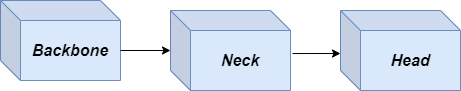
\includegraphics[scale=0.5]{images/objdet_structure.png}
  \caption{General neural network architecture for one-stage object detectors}
      \label{architecture}
\end{figure} 

The role of the backbone is to extract feature maps from the original image, that describe for instance various shapes which can help in determining the location and class of the possible objects. Depending on the precision and speed requirements the specific design of the backbone can vary from small networks, used for speed, or large networks, used for better precision. The actual design can be custom, but if there is not enough data to accommodate the required size of the network, a common practice is to use transfer learning. 

The idea is to use an already existent network architecture that is trained on a large amount of diverse data. Usually, a network used for classification is used by replacing the last layers with the neck and head architecture specific for the given problem. In this way, the extracted knowledge from the larger source dataset is stored in the network and it can be reused on the target dataset. How many layers are cut from the image classifier neural network depends on how similar are the target and source dataset. Also, regarding training, the first step is to train the whole network with the backbone frozen in order to not break the knowledge stored in its weights and the second step is to train the whole network with the backbone unfrozen, but with a low learning rate, in order to better fit the target dataset. For example a ResNet like architecture \cite{resnet} can be used if high precision is needed, or a MobileNet like architecture \cite{mobilenetv1, mobilenetv2} is suitable if speed is of the essence.

The neck is an optional component and its main role is to be an intermediary between the backbone and the head, such that it further refines the features from the backbone in order to provide more information for the head. An example for the neck architecture is the Feature Pyramid Network \cite{fpn}. The idea is that there are several feature maps extracted from the backbone that are provided to the head, in order to let the network to "see" at several resolutions.

If the other two components are not necessarily that specific to object detection, the head is responsible for taking the output of the neck (or directly from the backbone if the neck does not exist), optionally refine them furthermore, and finally converting them to the desired representation. This is the part where YOLO method contributes the most. Basically, it describes how the head should convert a feature maps into a representation from which bounding boxes can be extracted.

\subsection{YOLO head}

The main idea behind YOLO is that in order to detect multiple objects, at various locations, the image is split in a grid in which each cell is responsible for detecting objects that appear inside it. In fact, this is the representation of the ground truth labels.

\subsubsection{Ground truth definition}

The ground truth is represented as a $C \times C \times B \times (5+N)$ tensor. For each cell in the $C \times C$ grid, there are B anchor boxes associated. Each anchor box has the following parameters: $b_x$ and $b_y$ represent the center of the box and they are both relative to the cell responsible for predicting the object, meaning that they are divided to the size of the cell, $b_w$ and $b_h$ represent the width and height, c is the probability that the anchor predicts an object and $c_1, c_2, c_3, ... c_n$ represent the $N$ class probabilities, hence the $5+N$ term. The actual choice for the size of the grid, the number of anchors or the number of classes is problem specific. They are important because they determine the maximum number of positives in an image. The problem of defining positives in object detection is also an important concern.

When choosing anchors there are mainly two approaches. Either they are set by hand, or they are computed through a clustering algorithm over the whole dataset. The authors for example use K-Means, with one cluster per anchor, in order to better fit the patterns of the bounding boxes in the dataset. 

In the original version of the method, each cell is responsible for predicting only one bounding box, meaning that the idea of anchors is not used. As it's the case with many algorithms, anchors are only an optimization. Technically speaking, in ideal conditions, with enough data, it is enough to have one predictor per cell in order to regress any object. But as it it's often the case, there is not enough data, therefore, anchors were introduced for simplicity in the idea that it is good to split a complex problem in multiple simpler problems. The idea is that there are multiple predictors per cell that can learn various objects shapes. In this way, one predictor can specialize in tall objects and another in wide objects for instance. This also helps if there are multiple overlapped objects corresponding to one cell. 

In order to create the ground truth for an image, the bounding box labels must contain the center of the object, its width and its height. The way this information is expressed can vary, but it is not important as long as the center, width and height can be computed. The next step is to find the cell in which the center of the object falls into. That cell will be responsible for detecting the object. Then the anchor that is the closest to the object in terms of shape must be chosen. This is done using Intersection Over Union (IOU). 

\subsubsection{Interpretation of the raw output}

Regarding the network design, the final layer has the same structure as the ground truths. One way this can be implemented is with a 1x1 (pointwise) convolution. In order to do this, the layer before the pointwise convolution should output a feature map with a spatial size of $C \times C$. The number of channels does not matter because it is controlled by the pointwise convolution which has $B * (5 + N)$ kernels in order to output a feature map of size $C \times C \times (B * (5+N))$ which can be further reshaped to a tensor of shape $C \times C \times B \times (5+N)$ in order to match the shape of the ground truth.

The height, width and the coordinates of the object center are computed using the following formulas:
\begin{equation}
\begin{split}
    & bbox_x = \sigma(z_x) + c_x \\
    & bbox_y = \sigma(z_y) + c_y \\
    & bbox_w = a_w \cdot e^{z_w} \\ 
    & bbox_h = a_h \cdot e^{z_h} \\
    & bbox_obj = \sigma(z_{obj})
\end{split}
\label{conversion_formulas}
\end{equation}

The network predicts the raw values $z_x, z_y, z_w, z_h$. The upper left corner of the predicting cell is given by $c_x, c_y$ and are needed because the coordinates of the center are represented in the grid coordinate system. The width and height are relative to the predicting anchor, hence $a_w, a_h$ are used in computing the width and height of the object. Another value is predicted, that predicts the objectness $z_{obj}$ of the bounding box, meaning that it represents the probability that there is a bounding box predicted by the anchors. Also, the softmax can be used in order to get the class probabilities, which are further multiplied with the objectness score. In order to compute the loss it is enough to leave $bbox_x$ and $bbox_y$ as they are, but they are relative to the predicting grid cell and in order to get the actual bounding box relative to the image, $bbox_x$ and $bbox_y$ need to be multiplied with the size of the grid cell in order to get them in the coordindate system of the image.

As it is the case with most object detectors, YOLO can benefit from using Non-maximum Suppression. A common problem in object detection are the overlapping bounding boxes that actually predict the same object. The role of Non-maximum Suppression is to prune away extra bounding boxes. The first step is to order descending the bounding boxes by their objectness scores. The boxes are parsed one by one, and they are kept if the IOU with any bounding box of the same class previously kept is below a certain threshold. Hence only, the bounding box with the highest score will be kept in a certain region. As the object detectors become denser and denser, this operation becomes a very relevant one. There are also resarch interest in finding object detection methods that do not need this filtering due to its computational cost.


\subsection{Methodologies based on YOLO}

The success of the YOLO method is given by the robustness it has shown through time. Over the years, several methodologies have been proposed that use YOLO as the key element. Each brings different optimizations over the original method, but the main aspects are still relevant. For example, the second version of YOLO \cite{yolov2} mainly introduces the notion of anchors and a novel multi-scale training method in order to have good predictions across images of various scales. The third version of YOLO \cite{yolov3} represents mostly a bundle of small improvements. 

YOLO gained such a success that the original author has stopped its research in the field of artificial intelligence due to the fact that his work could be used to do harm, in modern warfare for example. In spite of this, the research into this method did not stop, because other people have developed several newer optimizations over the original algorithm. Also, this might be due to the fact that YOLO is very relevant in the industry of embedded computing, being a top choice for systems that have low resources and need to perform the task of object detection.

For instance, object detectors such as YOLOv7 \cite{yolov7} and YOLOX \cite{yolox} use the YOLO method in modern methodologies. The newer training techniques and optimizations resulted in competitive object detectors which achieve state of the art results. In YOLOX the authors propose an anchor free solution, and in YOLOv7 the authors continued an existing trend, that of finding methods that improve the performance without increasing the number of parameters, hence the speed loss is minimized.

The fact that there is still an ongoing research interest into this method is another argument for its success and robustness.